\NeedsTeXFormat{LaTeX2e}
\documentclass[11pt]{article}
\usepackage{url}
\usepackage{amsmath}
\usepackage{amsthm}
\usepackage{amssymb}
\usepackage{mathpartir}
\usepackage{graphicx}
\usepackage{comment}


\newcommand{\deftech}[1]{\textbf{#1}}
\newcommand\mrel{\mathop{\mathbf{r}}}
\newcommand\morel{\mathop{\mathbf{r}'}}
\newcommand\menv{\rho}
\newcommand\mval{v}
\newcommand\mans{a}
\newcommand\mint{i}
\newcommand\moint{j}
\newcommand\mbool{b}

\newcommand\plug[2]{#1[#2]}

\newcommand\merr{r}

\newcommand\mctx{\mathcal{C}}
\newcommand\mectx{\mathcal{E}}
\newtheorem{theorem}{Theorem}
\newcommand\Err{\mathit{Err}}
\newcommand\Plus{\mathit{Plus}}
\newcommand\Mult{\mathit{Mult}}
\newcommand\Succ{\mathit{Succ}}
\newcommand\Pred{\mathit{Pred}}
\newcommand\Eq{\mathit{Eq}}
\newcommand\True{\mathit{True}}
\newcommand\False{\mathit{False}}
\newcommand\If{\mathit{If}}
\newcommand\Div{\mathit{Div}}

\newcommand\reduce{\mathop{\mathbf{b}}}

\newcommand\areducename{\mathbf{a}}
\newcommand\areduce[2]{#1\;\areducename\;#2}

\newcommand\step{\rightarrow_\mathbf{b}}
\newcommand\multistep{\rightarrow^\star_\mathbf{b}}

\newcommand\astdstep{\longmapsto_{\reduce}}
\newcommand\astdmultistep{\longmapsto^\star_{\reduce}}

\newcommand\breducename{\mathbf{b}}
\newcommand\errreducename{\mathbf{err}}
\newcommand\propreducename{\mathbf{prop}}
\newcommand\bvreducename{\mathbf{bv}}
\newcommand\bstepname{\rightarrow_{\breducename}}
\newcommand\bmultistepname{\rightarrow^\star_{\breducename}}

\newcommand\bmultistep[3]{#1\vdash #2\;\bmultistepname\;#3}
\newcommand\bstdstep[3]{#1\vdash #2\;{\longmapsto_{\breducename}}\;#3}
\newcommand\bstdmultistep[3]{#1\vdash #2\;{\longmapsto^\star_{\breducename}}\;#3}

\newcommand\breduce[3]{#1 \vdash {#2}\;\breducename\; {#3}}
\newcommand\errreduce[3]{#1 \vdash {#2}\;\errreducename\; {#3}}
\newcommand\propreduce[3]{#1 \vdash {#2}\;\propreducename\; {#3}}
\newcommand\bvreduce[3]{#1 \vdash {#2}\;\bvreducename\; {#3}}
\newcommand\bstep[3]{#1 \vdash {#2}\;\rightarrow_{\breducename}\; {#3}}
\newcommand\bclosedstep[2]{{#1}\;\rightarrow_{\breducename}\; {#2}}

\newcommand\laxparstep{\rightrightarrows_\mathbf{a}}
\newcommand\maxparstep{\rightrightarrows'_\mathbf{a}}


\newcommand{\xdown}[1]{X_{#1 \downarrow}}
\newcommand{\xup}[1]{X_{#1 \uparrow}}
\newcommand{\xdownk}[2]{X_{#1 \downarrow #2}}
\newcommand{\xupk}[2]{X_{#1 \uparrow #2}}
\newcommand{\xblock}[1]{[x_{#1 1}, x_{#1 2} , \dots, x_{#1 \frac{1}{c}}]^{\top}}
\newcommand{\conpr}[2]{Pr[#1\,|\,#2]}
\newcommand{\priv}{{\bf priv}(X)}
\newcommand{\alt}[1]{{\bf alt}(X_{#1})}
\newcommand{\xbot}[1]{x_{#1 \frac{1}{c}}}
\newcommand{\cwp}[1]{(\epsilon, \delta, \Delta_{#1}, \Gamma)}


\newcommand\Arith{\mathcal{A}}
\newcommand\Barith{\mathcal{B}}

\newcommand\Var{\mathit{Var}}

\newcommand{\mvar}{x}
\newcommand\s[1]{\mathit{#1}}

\title{Streaming CW-Pivacy}
\date{\today}
\begin{document}
\maketitle
\section{Streaming Setting 1}
\begin{figure}[th]
\centering
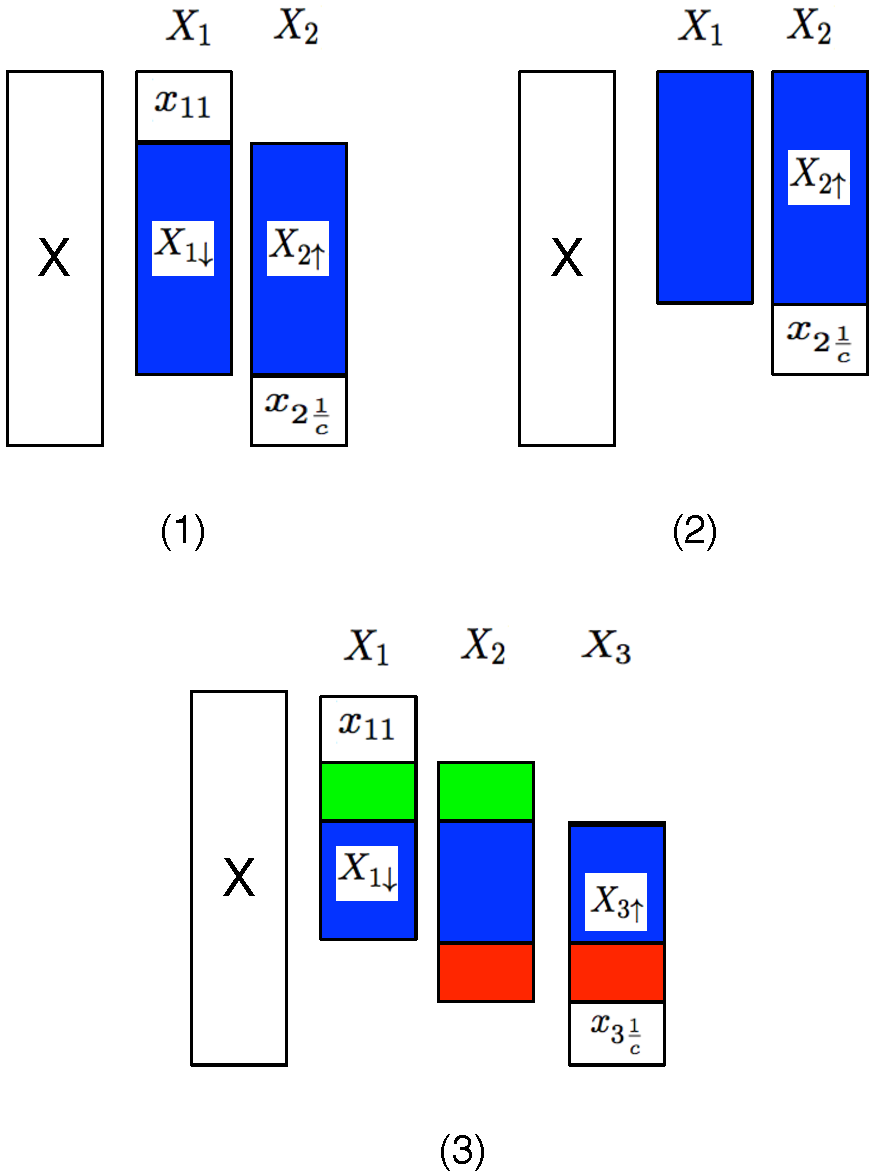
\includegraphics[width=4.5in]{fig/stream_database3.pdf}
\caption{\label{stream_db3} Blocks in color are shared by more than one databases. Blocks in white are owned by only one database. (1) Composition of $F(X_{1})$ and $F(X_{2})$. It has ``good" independence since each $X_{i}$ owns one block. (2) Composition of $F(X_{1})$ and $F(X_{2})$ with $X_{1}$ to be a part of $X_{2}$. (3) Composition of queries on three streaming databases. Cannot leverage ``good" independence.}
\end{figure}
\begin{figure}[th]
\centering
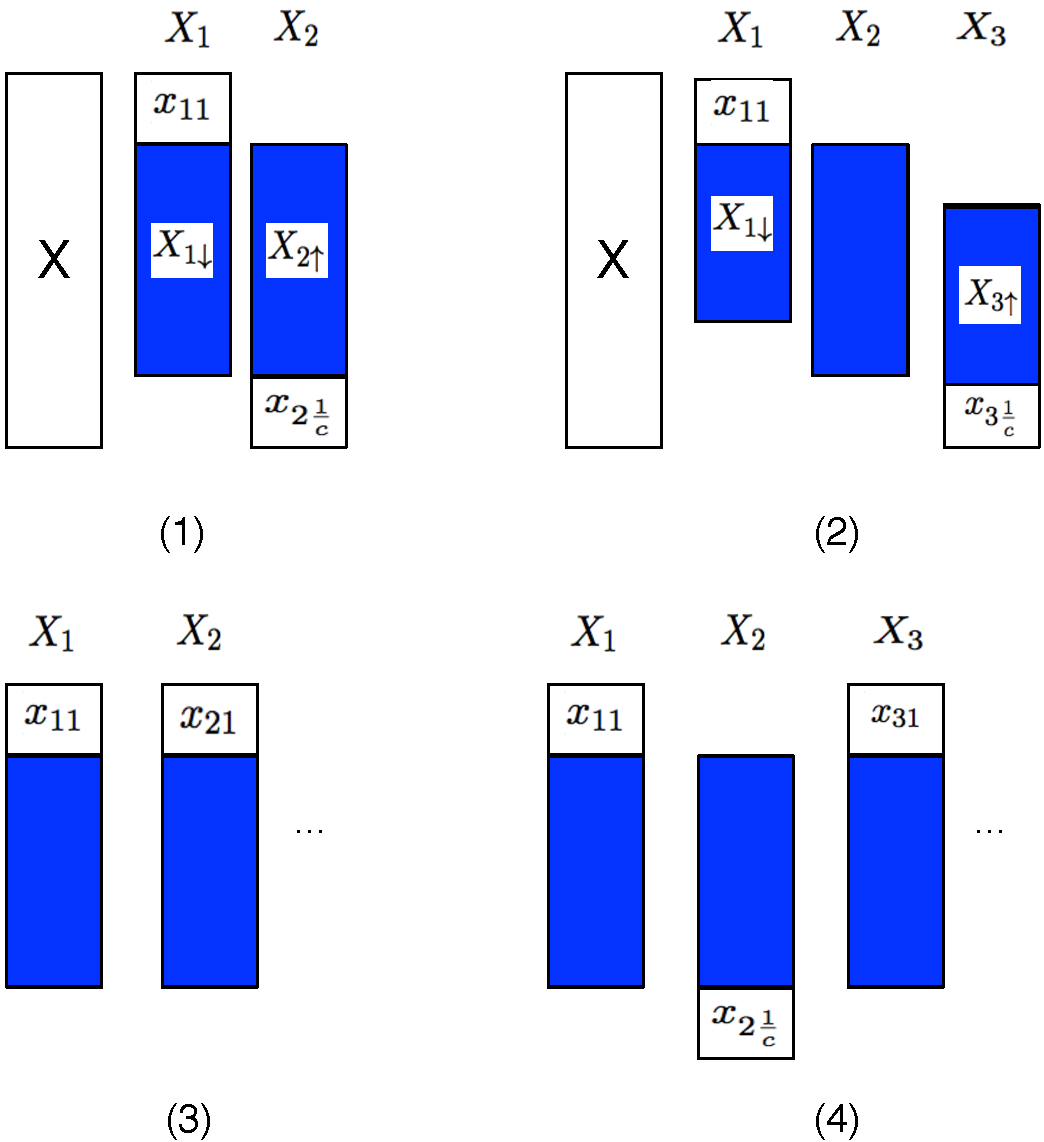
\includegraphics[width=4.8in]{fig/stream_database1.pdf}
\caption{\label{stream_db1} Blocks in blue are shared by more than one databases. Blocks in white are owned by only one database. (1) Composition of $F(X_{1})$ and $F(X_{2})$. It has ``good" independence since each $X_{i}$ owns one block. (2) Composition of queries on three streaming databases. Cannot leverage ``good" independence, because each block in $X_{2}$ is shared by two databases. (3) Composition of queries in the standard DP case. The blue blocks refer to the query while the white blocks refer to the independent noise. (4) It works as long as each streaming database owns one block of ``private" block.}
\end{figure}
\begin{figure}[th]
\centering
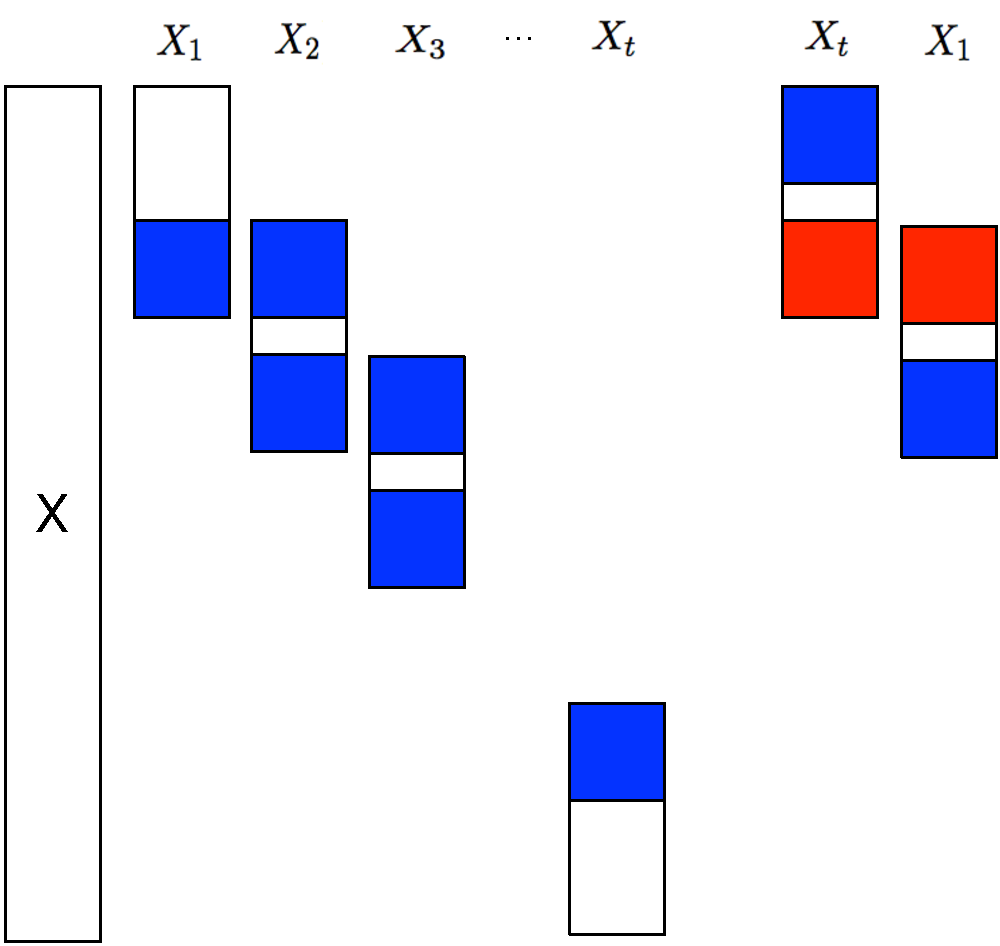
\includegraphics[width=4.8in]{fig/stream_database2.pdf}
\caption{\label{stream_db2} Blocks in blue are shared by more than one databases. Blocks in white are owned by only one database. Construct streaming databases such that each $X_{i}$ owns a block of $cn$ rows by itself. In this figure, the middle block is always private. At each time step, $\frac{1+c}{2} n$ rows need to be generated independently. We can connect $X_{t}$ back to $X_{1}$ to make the big database $X$ circular. Now, $X$ has size of  $\frac{1+c}{2} nt$}
\end{figure}

{\bf Problem setting} \\
Let $X$ be a database in the streaming setting. Let $X_{i}$ represent the portion of $X$ that is currently held at time step $i$. We assume that at each time step, a fraction of $c$ of the database is replaced. We assume the oldest rows are always the ones replaced, and that $X$ has row drown i.i.d. from some distribution $D$. Let $n$ be the size of each $X_{i}$. This means that the first $n$ rows of $X$ constitute $X_{1}$, rows $cn+1$ through $cn+n$ constitute $X_{2}$, and so forth. $X$ has size $n+cn(t-1)$, where $t$ is the total number of time steps being considered. $1/c$ is the total number of time steps a given row will be present for. See (1) and (2) in Figure~\ref{stream_db1}. 
\\
\\
{\bf Hypothesis}\\
We now consider a query $F: \, {\cal U}^{n} \rightarrow \mathbb{R}^{d}$ on each $X_{i}$. 
Let $D_{F}$ be the distribution that draws a database of size $n$, with each row chosen i.i.d. from $D$. Let $aux_{F}$ be $F$'s auxiliary information, which consists of any $(1-c)n$ rows of the database. Now, assume $F$ is $(\epsilon, \delta, \Delta_{F}, \Gamma)$-CW private with some simulator $sim_{F}$, where $\Delta$ chooses the database according to $D_{F}$ and the auxiliary information is $aux_{F}$ as stated above.

Let $G(X) = (F(X_{1}), F(X_{2}) , \dots, F(X_{t}))$ be the composite query that runs $F$ at each time step. We show $G$ is $(? \epsilon, ? \delta, \Delta, \Gamma)$ -CW private.
\\
\\
{\bf Notations }\\
For each $X_i$ of size $n$, we represent it by $1/c$ blocks (each has $cn$ rows). Namely, let $X_{i}=\xblock{i}$, where $x_{ij}$ denote the $j$th block in $X_{i}$. Let $\xdownk{i}{k} = [x_{i (k+1)}, x_{i (k+2)} , \dots, x_{i \frac{1}{c}}]^{\top}$ and $\xupk{i}{k} = [x_{i 1}, x_{i2} , \dots, x_{i (\frac{1}{c}-k)}]^{\top}$. We use $\xdown{i}$ to denote $\xdownk{i}{1}$ and $\xup{i}$ to denote $\xupk{i}{1}$. Notice that $\xdownk{i}{k} = \xupk{i+k}{k}$ (specifically $\xdown{i} = \xup{i+1}$), which are the shared blocks between $X_{i}$ and $X_{i+k}$. See (1) and (2) in Figure~\ref{stream_db1}.

Let $S=(S_{1}, S_{2}, \dots, S_{t} )$ be any set from $\mathbb {R} ^{d \times t}$, where $S_{j}$ is determined by the values of $(s_{1}, s_{2} , \dots, s_{j-1})$. Let $S_{-t}$ denote set $(S_{1}, S_{2}, \dots, S_{t-1} )$.
\\
\\
{\bf The cases $\&$ when it does (does not) work}\\
The base case is when $G(X) = (F(X_{1}) , F(X_{2}))$. See (1) in Figure~\ref{stream_db3}.
\begin{enumerate}
\item In case (1), it is not hard to show $G(X)$ is $(2 \epsilon, 2 \delta, \Delta, \Gamma)$ -CW private, with simulator $(sim_{F}, sim_{F})$. Please refer to previous write-up for the proof. We can even prove $G(X)$ is $(2 \epsilon, 2 \delta, \Delta, \Gamma)$ -CW private, given the common blocks shared by $X_{1}$ and $X_{2}$.
\item In case (2) (we talked about it last Thursday), $X_{1}$ is a subset of $X_{2}$ with $X_{2}$ has a fraction of new blocks. It appears that this case {\bf does not work}.

Following the proof for the base case (or Adam's proof in page 46-47), we can get the follows: For any set $S=(S_{1}, S_{2})$,
\[
Pr [G(X) \in S] \leq e^{\epsilon}  Pr({sim_{F}(\alt{2}) \in S{2}}, { F(X_{1}) \in S_{1}})+\delta.
\]
But it appears that we still need to leverage the independence of $F(X_{1})$ w.r.t. $sim_{F}(\alt{2})$. That is, we need to considering the following equation.
\[
Pr({sim_{F}(\alt{2}) \in S{2}}, { F(X_{1}) \in S_{1}}) 
\]
\[
= \conpr{F(X_{1}) \in S_{1}}{sim_{F}(\alt{2}) \in S{2}} \cdot Pr[sim_{F}(\alt{2}) \in S{2}]
\]
Since every row in $X_{1}$ is also in $X_{2}$, we do not have any type of independence. In fact, we really need a fraction of rows in $X_{1}$ that are independent of $X_{2}$ to proceed from here.
\item Consider the case when compose three queries. See case (3) in Figure~\ref{stream_db3}. Similarly, we get the following step.
\[
Pr [G_{3}(X) \in S] \leq e^{\epsilon}  Pr({sim_{F}(\alt{3}) \in S{3}}, { F(X_{2}) \in S_{2}}, { F(X_{1}) \in S_{1}})+\delta
\]
Next, we have to consider the following conditional probability.
\[
Pr({sim_{F}(\alt{3}) \in S{3}}, { F(X_{2}) \in S_{2}}, { F(X_{1}) \in S_{1}}) =
\]
\[
\conpr{G_{2}(X) \in (S_{1}, S_{2})} { sim_{F}(\alt{3}) \in S{3}} \cdot Pr[sim_{F}(\alt{3}) \in S{3}].
\]
Now, we need to leverage a type of independence between $G_{2}(X)$ and $sim_{F}(\alt{3})$. The common blocks of $X_{3}$ and $X_{1} \cup X_{2}$ are $\xup{3}$ (the blue and red blocks in (3) of the Figure~\ref{stream_db3}). We need to consider the total conditional probability on the value of $\xup{3}$.
\[
\conpr{G_{2}(X) \in (S_{1}, S_{2})} { sim_{F}(\alt{3}) \in S{3}} 
\]
\[
=\Sigma_{z} \conpr{G_{2}(X) \in (S_{1}, S_{2})} { sim_{F}(\alt{3}) \in S{3}, \xup{3}=z} \cdot Pr[ \xup{3}=z] 
\]
Given $\xup{3}=z$, $G_{2}(X)$ is independent with $sim_{F}(\alt{3})$. However, $G_{2}(X)$ is not CW-private given $\xup{3}$ as the auxiliary information (red+blue blocks). The problem here is: every block in $X_{2}$ is either shared with $X_{1}$ (blue+green blocks), or given in the auxiliary information (red blocks). Just like the case 2 above, we cannot leverage a type of independence between $X_{1}$ and $X_{2}$.
\end{enumerate}

\end{document}
